%!TEX root = ../2019_06_04-HATS-LPC-JEC.tex

\subsection{Analysis Requirements}
\label{sec:analysis}
%---------------------------------------------------------------------------------------------------------------------------------------
\frame{
\frametitle{Mandatory Jet Energy Corrections at CMS}
%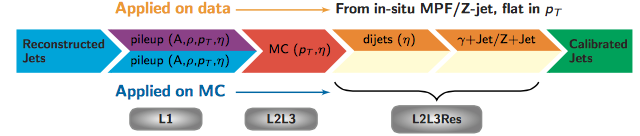
\includegraphics[width=10cm]{images/jecs.png}
\begin{itemize}
\item The minimum correction levels to be applied on any CMS analysis using Monte Carlo and Data are:

\begin{itemize}
\item \textbf{Monte Carlo:}\\
{\color{red}L1(Pile Up) + L2(Relative) + L3(Absolute)}
\item \textbf{Data:}\\
{\color{red}L1(Pile Up) + L2(Relative) + L3(Absolute) + L2L3 Residuals}
\end{itemize}
\item Any analysis might place higher correction levels if necessary and available. 
\item User can check \href{https://twiki.cern.ch/twiki/bin/view/CMS/JECDataMC}{https://twiki.cern.ch/twiki/bin/view/CMS/JECDataMC} to learn about the ``Recommended Jet Energy Corrections and Uncertainties for Data and MC".
\item The use of JER scale factors is also usually required. Directions for those can be found at \href{https://twiki.cern.ch/twiki/bin/view/CMS/JetResolution}{https://twiki.cern.ch/twiki/bin/view/CMS/JetResolution}
\end{itemize}

}
%---------------------------------------------------------------------------------------------------------------------------------------
%\subsubsection{JER Uncertainty Sources}
%\frame{
%\frametitle{JES and Uncertainties}
%\begin{block}{Description}
%\begin{itemize}
%\item The JEC uncertainty sources provide detailed information on JEC uncertainties for use in statistical data analysis. The sources are fully uncorrelated between themselves, but describe JEC variations that are fully correlated within a given source.
%\item FIX ME: Should we include how uncertainties are calculated? How they are applied? Sources?
%\end{itemize}
%\end{block}
%}
%---------------------------------------------------------------------------------------------------------------------------------------
\subsection{Collections}
\frame{
	\frametitle{Jet Collections Supported by the JERC Group}
	\begin{itemize}
		\item Clustering algorithms:
		\begin{itemize}
			\item Anti-k$_{T}$
		\end{itemize}
		\item Cone sizes:
		\begin{itemize}
			\item R=0.4, 0.8
		\end{itemize}
		\item Jet types:
		\begin{itemize}
			\item PF - Still in use
			\item PF+CHS - Still used in some cases
			\item PF+PUPPI - More and more becoming the default
			\item Calo - Mostly used as a backup (for comparison)
			\item Jet Plus Track (JPT) - Expert use only
		\end{itemize}
	\end{itemize}
}
%---------------------------------------------------------------------------------------------------------------------------------------
\subsection{JEC Release Procedure}
\frame{
	\frametitle{JEC Release Procedure}
	\begin{itemize}
          \item Announced on ``JetMET: Jet Energy Scale'' hypernews
          \item Described on \href{https://twiki.cern.ch/twiki/bin/view/CMS/JECDataMC}{{\color{blue}https://twiki.cern.ch/twiki/bin/view/CMS/JECDataMC}}
          \item {Important to read the ``Notes'' associated to an update, which often describe only partial updates}

                \begin{figure}
                  \scalebox{.9}{
                          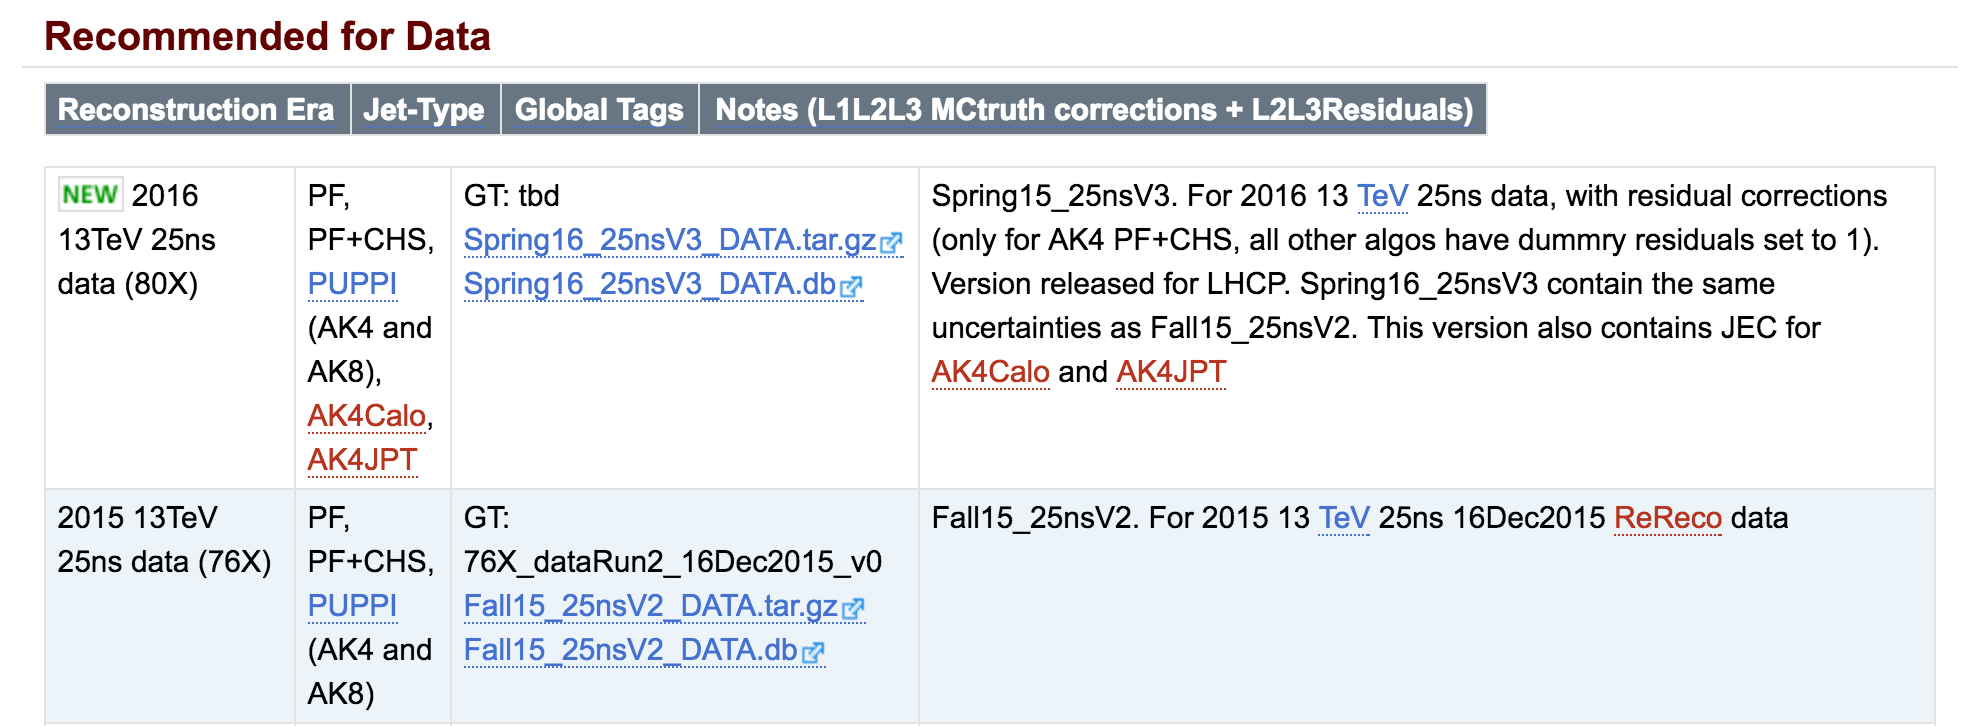
\includegraphics[width=\textwidth]{images/jec_twiki.png}
                        }
                \end{figure}

	\end{itemize}
}